\chapter{Introduzione e Definizione del Problema}

L'\textbf{anomaly detection} (o outlier detection), è il processo che mira ad identificare i dati che deviano in modo significativo dalla maggioranza delle osservazioni, portando a presupporre che siano generati da un meccanismo differente. 

Individuare queste irregolarità comporta sfide uniche dovute alla natura intrinseca del problema. Tra le principali complessità sono presenti:
\begin{itemize}
    \item l'incognita delle anomalie: le anomalie rimangono sconosciute finché non si verificano.
    \item l'eterogeneità delle anomalie: le diverse classi di anomalie possono avere caratteristiche totalmente diverse tra loro.
    \item la rarità delle anomalie: vi è un grande squilibrio di classe rispetto la maggioranza di dati normali. \cite{Pang_et_al._2021}
\end{itemize}

Il processo di rilevamento delle anomalie ha una lunga storia, costituita da studi e applicazioni di metodologie sempre più innovative che puntano alla risoluzione delle molteplici sfide che caratterizzano la materia.
Le principali per le quali le tecnologie moderne, in particolare il deep learning, giocano un ruolo fondamentale sono:

\begin{enumerate}
    \item \textbf{Basso tasso di richiamo (Recall)}: data la rarità e l'eterogeneità delle anomalie, alcuni metodi possono generare dei "falsi positivi". La sfida è quella, quindi, di ridurre i falsi positivi, aumentando le capacità di individuare le vere anomalie.
    \item \textbf{Dati ad alta dimensionalità e interdipendenti}: le anomalie, evidenti in poche dimensioni, tendono a scomparire all'aumentare della complessità dei dati. Inoltre, risulta sfidante individuare anomalie quando le istanze sono interdipendenti tra loro.
    \item \textbf{Apprendimento efficiente con pochi dati}: ottenere grandi quantità di dati anomali spesso è costoso e poco pratico. La sfida è riuscire a massimizzare lo sfruttamento dei dati parzialmente etichettati per poter distinguere i dati normali dalle anomalie e quindi generalizzare il modello anche per anomalie mai viste prima.
    \item \textbf{Resilienza al rumore}: i dati di addestramento reali non sono quasi mai perfettamente puliti, ma anzi spesso contengono etichette errate o anomalie non classificate. Sorge necessario sviluppare modelli capaci di tollerare, o ancor meglio sfruttare questi dati.
    \item \textbf{Rilevamento di anomalie complesse}: la maggior parte dei sistemi classici è addestrata in modo tale da concentrarsi su singole anomalie puntuali, è necessario espandere il rilevamento ad anomalie contestuali o collettive. La sfida è quella di creare, quindi, modelli capaci di ricordare il contesto e valutare interi gruppi di dati.
    \item \textbf{Spiegabilità (Anomaly Explanation)}: spesso i modelli complessi agiscono come scatole nere. Oltre a rilevare un'anomalia, il sistema deve fornire delle motivazioni che siano interpretabili. Questa "trasparenza" è fondamentale per garantire affidabilità (soprattutto in domini critici), permettere la supervisione umana e garantire l'ottimizzazione del modello bilanciando potenza e verificabilità.
\end{enumerate} 

L'applicazione di metodi basati sul deep learning riesce quindi a superare i limiti dei metodi più tradizionali, ottimizzando il processo interamente e apprendendo rappresentazioni specifiche per il rilevamento di anomalie. Riescono a sfruttare dati parzialmente etichettati, complessi e anche ad alta dimensionalità, unificando il rilevamento e la spiegazione in un unico sistema.

\section{L'anomaly detection nella Computer Vision}

La Visual Anomaly Detection (VAD) è un punto cruciale nel campo del machine learning e della computer vision in quanto l'obiettivo è identificare, all'interno di dati visivi come ad esempio immagini o nuvole di punti, ciò che devia rispetto ad un concept stabilito di "normalità". \cite{Cao_et_al._2024}
Rispetto alla maggior parte dei metodi di machine learning classici, che assumono di operare in un sistema statico e chiuso, in cui tutte le classi sono note a priori; la VAD studia come i modelli possano gestire informazioni sconosciute e incerte in un ambiente aperto e dinamico. \cite{Yang_et_al._2021}

A seconda del grado di ispezione, la VAD si divide in \textbf{image-level}, stabilendo se l'intera immagine è anomala e \textbf{pixel-level}, in cui viene localizzata l'esatta regione del difetto, rivelandosi vitale in campi come l'ispezione di difetti industriali, identificazione di lesioni mediche e rilevamento di ostacoli nella guida autonoma. \cite{Yang_et_al._2021}\cite{Pang_et_al._2021}.

    
\subsection{Sfide Principali dell'Anomaly Detection}

Negli ultimi anni, l'integrazione di sistemi intelligenti e dell'Internet of Things (IoT) all'interno dei processi industriali ha contribuito a generare una mole di dati senza precedenti. In questo contesto, garantire l'integrità, la sicurezza e l'affidabilità dei dati è un requisito fondamentale per garantire continuità operativa. 
Il rilevamento delle anomalie, diventa centrale per far fronte a questa necessità, configurandosi come strumento cardine per identificare tempestivamente guasti meccanici, difetti di produzione, o minacce informatiche prima che diventino fermi macchina o rischi per la sicurezza.
Nonostante i grandi successi del Deep Learning e del Machine Learning in scenari controllati, trasferire queste tecnologie in realtà operative presenta ostacoli non banali.\cite{Aggarwal_et_al._2021}\cite{Yang_et_al._2023}\cite{Ren_et_al._2021}

Per riuscire a progettare soluzioni robuste e dispiegabili sul campo, risulta indispensabile analizzare tre sfide principali:

\begin{enumerate}
    \item Sbilanciamento delle classi.
    
    I dataset, in particolare quelli industriali, presentano una rarità di dati anomali rispetto a quelli che definiscono il normale funzionamento. 
    In linee di produzione efficienti, infatti, i dati relativi ai guasti sono estremamente sporadici. 
    Questa asimmetria estrema rende approcci classici spesso inefficaci. Essi, infatti, tendono a soffrire di un bias sistematico verso la classe maggioritaria (quella normale), non riuscendo a generalizzare e riconoscere i rari eventi critici.\cite{Yang_et_al._2023} \cite{Aggarwal_et_al._2021}

\begin{figure}[htbp]
    \centering
    % Sbilanciamento_delle_classi
    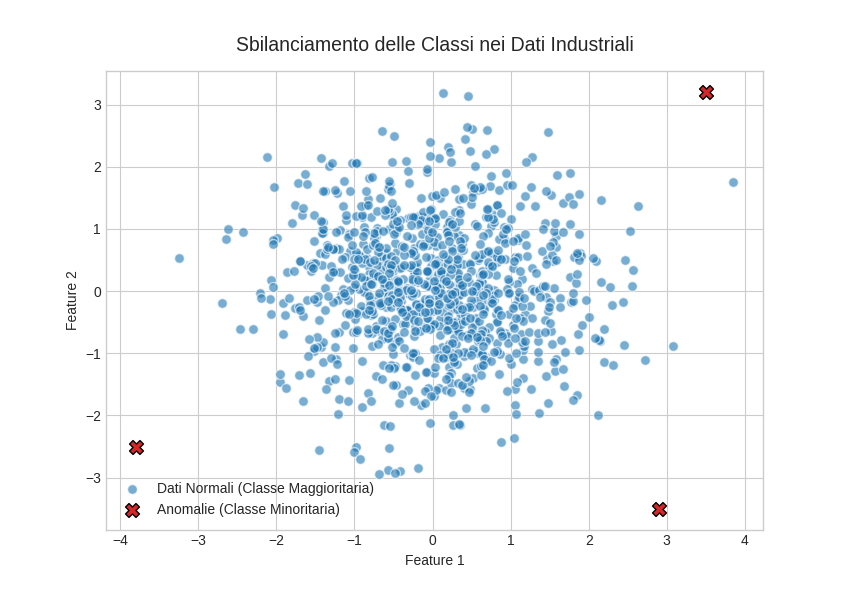
\includegraphics[width=0.8\textwidth]{Sbilaciamento_delle_classi.png}
    \caption{Rappresentazione dello sbilanciamento estremo tra dati di normale funzionamento e rari eventi anomali.}
    \label{fig:sbilanciamento}
\end{figure}

    
    \item Variabilità ed eterogeneità dell'anomalia.

    Le anomalie presentano caratteristiche di estrema eterogeneità e una natura senza confini definiti. Un malfunzionamento non si manifesta quasi mai secondo un pattern identico, ma anzi può configurarsi come un picco improvviso, un comportamento collettivo anomalo o un'anomalia contestuale.
    Poiché i guasti sono infinitamente diversificati, risulta impossibile poter mappare tutte le possibili configurazioni di anomalia all'interno di un singolo modello. Per questo, l'algoritmo deve possedere una spiccata capacità di astrazione, riuscendo a catalogare come anomalia qualsiasi entità fuori dallo spazio "normale" anche se mai vista in addestramento.\cite{Yang_et_al._2023} \cite{Aggarwal_et_al._2021}\cite{Ren_et_al._2021}

\begin{figure}[htbp]
    \centering
    % Variabilità dell'anomalia
    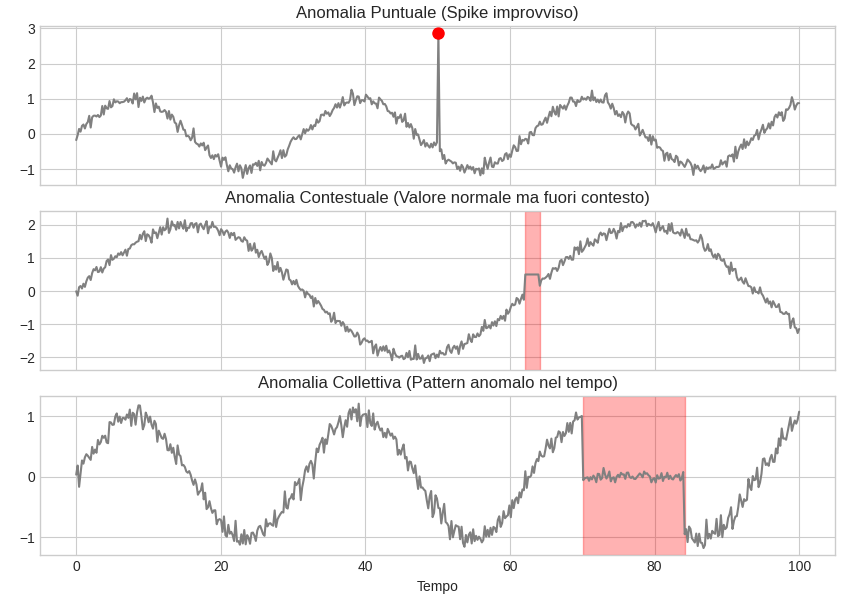
\includegraphics[width=0.8\textwidth]{Variabilita_dell_anomalia.png}
    \caption{Rappresentazione delle tre diverse tipologie di anomalia in una serie temporale: puntuale, contestuale e collettiva.}
    \label{fig:variabilita_anomalia}
\end{figure}


    \item Vincoli e complessità dei contesti industriali.

    I dati sensoriali di una fabbrica sono strettamente legati ad una forte dipendenza del contesto. Un determinato valore di vibrazione o di temperatura può essere considerato perfettamente normale in un determinato momento, come ad esempio, in una particolare stagione, o in una determinata fase produttiva, ma può essere considerata un'anomalia in altri momenti.
    I confini tra anomalia e normalità, sono sfumati e ambigui. I campioni presentano spesso fluttuazioni insolite, dovute a tolleranze industriali che potrebbero ricalcare i tratti delle anomalie, generando falsi positivi.
    Il modello deve, quindi, essere progettato con l'integrazione di feature contestuali per evitare che il modello risulti rigido e non adattabile ai cambi di scenario. Diventa fondamentale riuscire ad implementare una fase di pre-elaborazione per mitigare l'effetto dei disturbi sensoristici.\cite{Yang_et_al._2023} \cite{Aggarwal_et_al._2021}\cite{Ren_et_al._2021}

\begin{figure}[htbp]
    \centering
    % Vincoli e contesti industriali
    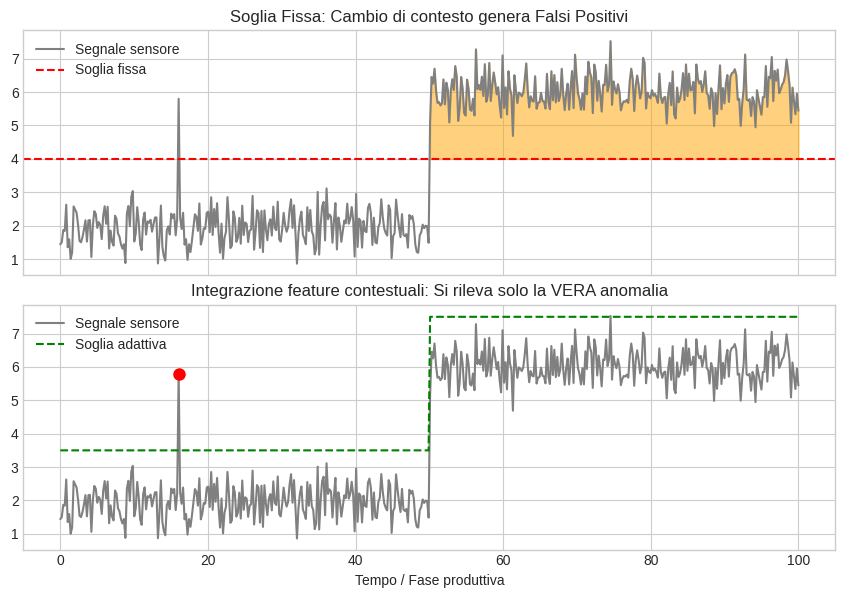
\includegraphics[width=0.8\textwidth]{Soglia_fissa_adattiva.png} % o .png
    \caption{Confronto tra l'uso di una soglia di anomalia fissa (che genera falsi positivi al cambio di fase produttiva) e una soglia adattiva basata sul contesto.}
    \label{fig:contesto_industriale}
\end{figure}
    
\end{enumerate}
 


\subsection{Definizioni dei Paradigmi}

Le sfide appena descritte — in particolare la rarità dei difetti e l'imprevedibilità del contesto industriale — rendono impossibile l'adozione di un'unica architettura universale. A seconda della disponibilità, della qualità e della mole di dati raccolti, la progettazione del modello deve adattarsi seguendo approcci di addestramento differenti. Vengono, quindi, definiti tre principali paradigmi che hanno guidato lo sviluppo delle metodologie di Visual Anomaly Detection. \cite{Yang_et_al._2021}

\begin{itemize}
    \item \textbf{Paradigma Supervisionato (Supervised Visual Anomaly Detection)}
    
    Il modello supervisionato (o apprendimento supervisionato) si basa su un paradigma fondamentale: l'algoritmo impara a compiere una determinata associazione o previsione partendo da un dataset di addestramento strutturato in \textbf{coppie di input e output attesi (etichette o labels)}.
    Questo paradigma funziona tramite una guida diretta:
    \begin{itemize}
        \item \textbf{Presenza di etichette (Labels):} ogni dato di input è associato ad una risposta corretta definita da un supervisore umano. Il modello viene quindi addestrato esplicitamente a riconoscere il difetto e a classificarlo come tale.
        \item \textbf{Definizione dei Confini di Classe:} ricevendo input di entrambe le categorie (buone e difettose), il modello supervisionato riesce a definire i confini decisionali (class boundaries) con estrema precisione, riducendo falsi allarmi e identificando esattamente un oggetto conforme da un non conforme.\cite{Beitieval_et_al._2024}
    \end{itemize}

    Le etichette sono soggette a differenti livelli di granularità in base al diverso metodo applicato. Nella supervisione a livello di immagine (Weakly Supervised) viene fornito solo un flag booleano (ad esempio 0 per sano, 1 per difettoso); mentre, nella supervisione a livello di Pixel (Pixel-level Supervised), viene richiesto uno sforzo umano più minuzioso, in quanto è necessario il disegno di maschere millimetriche attorno ad ogni singolo difetto. Quest'ultimo metodo, è molto potente ma estremamente costoso e lento e spesso impraticabile in contesti complessi.
    Nonostante l'elevata accuratezza del modello a livello teorico, però, i paradigmi supervisionati presentano ostacoli molto impattanti quando applicati a scenari reali.
    Essi, difatti, necessitano di grandi quantità di dati che siano esemplificativi per ogni classe; tuttavia, nelle linee di produzione reali, i difetti non sono così numerosi. Il modello finisce per andare in \textbf{overfitting}: a causa di dataset di training sbilanciati, con una presenza minima di difetti, il modello memorizza perfettamente i difetti visionati, ma perde la capacità di generalizzare.
    I difetti sconosciuti, in questo modo, verranno classificati come "sani" solamente a causa di una non conformità con i difetti appresi.\cite{Beitieval_et_al._2024}
\end{itemize}


\begin{itemize}
    \item \textbf{Paradigma non Supervisionato (Unsupervised Visual Anomaly Detection)}
    
    L'approccio non supervisionato consente di costruire modelli di rilevamento senza dover fare affidamento ad etichette o campioni annotati. In questo scenario, infatti, non sono presenti dati che addestrino il modello anticipandogli cosa sia "normale" e cosa sia "difettato". \cite{Cui_et_al._2023}
    Il paradigma non supervisionato si basa su alcune premesse fondamentali:
    \begin{itemize}
        \item scarsità statistica delle anomalie: si assume, come visto anche in precedenza, che le anomalie sia rare e minoritarie;
        \item differenziazione della norma: l'obiettivo non è raggruppare oggetti simili, ma determinare i campioni che sono più distanti o differenti dalla maggioranza dei dati;
        \item deviazione dal pattern: l'identificazione dell'anomalia avviene perché non sufficientemente simile al resto dei dati, e la differenza è misurata tramite specifiche caratteristiche, le \textbf{feature}.\cite{Guthrie_et_al._2007}
    \end{itemize}
    L'approccio non supervisionato presenta alcuni vantaggi, tra cui sicuramente l'abbattimento di tempi e costi. Non sorge, difatti, la necessità di etichettare manualmente e capillarmente i campioni. Un ulteriore vantaggio è il rilevamento delle anomalie sconosciute, in quanto esse vengono riconosciute attraverso l'analisi della differenza tra il campione e il modello di "normalità".\cite{Cui_et_al._2023} Il modello si presenta, inoltre, robusto rispetto alla contaminazione dei dati, riuscendo ad isolare e apprendere la normalità anche in presenza di dataset "sporchi".\cite{Lin_et_al._2021}
\end{itemize}


\begin{itemize}
    \item \textbf{Paradigma Semi-Supervisionato (Semi-Supervised Anomaly Detection)}
    Il modello semi supervisionato utilizza un set di addestramento che contiene esclusivamente istanze etichettate della classe "normale". Non è necessario quindi possedere delle etichette per la classe delle anomalie.
    Questo paradigma, risulta anch'esso essenziale data la nota rarità di anomalie e istanze "non normali".
    Per far fronte a queste necessità, si utilizzano tecniche a singola classe, che definiscono un confine decisionale, un \textbf{boundary}, attorno alla classe negativa, permettendo di isolare la regolarità dei dati normali rispetto gli anomali.
    Questo metodo, consente di rilevare tipologie di anomalie inedite che non erano mai apparse durante l'addestramento.
    Gli algoritmi che seguono questo paradigma si suddividono in due categorie principali:
    \begin{itemize}
        \item individuali: operano come modelli singoli. Tra le logiche che caratterizzano questi modelli possiamo distinguere i \textit{modelli lineari}, quelli \textit{basati sulla prossimità}, i \textit{modelli probabilistici}, e le \textit{reti neurali}.
        \item ensemble: riunisce e fonde più logiche sfruttando i risultati di molteplici classificatori individuali. La regola alla base è che una collezione di classificatori quasi identici non potrà mai superare le prestazioni dei suoi singoli componenti. Esempi possono essere \textit{l'isolation forest} e \textit{l'extreme gradient boosting outlier detection}.
    \end{itemize}
    Il paradigma presenta sicuramente vantaggi quali la scoperta di anomalie conosciute (Zero-Day) e l'efficacia in casi di sbilanciamento delle classi. Allo stesso tempo però, il modello è sensibile al "rumore" nei dati e potrebbe presentare un degrado delle prestazioni in contesti specifici, come ad esempio l'elaborazione di dati esclusivamente con feature di tipo nominale.\cite{Perez_et_al._2021}
\end{itemize}
\vspace{1em}

In sintesi, l'analisi dei paradigmi di apprendimento evidenzia come la scelta dell'approccio dipenda strettamente dalla natura e dalla disponibilità dei dati industriali. Sebbene i metodi supervisionati offrano un'elevata precisione, la rarità intrinseca delle anomalie spinge la ricerca verso soluzioni semi-supervisionate, capaci di modellare la "normalità" in modo flessibile e resiliente. Tuttavia, la sola definizione del paradigma non è sufficiente a garantire il successo in contesti operativi complessi. Risulta quindi fondamentale analizzare come queste logiche siano state declinate concretamente all'interno della letteratura scientifica recente. 


\section{Il Benchmark MVTec AD e le Metriche di valutazione}

Al fine di validare l'efficacia degli algoritmi di \textit{Anomaly Detection} nel contesto industriale, è indispensabile avere un quadro sperimentale standardizzato e condiviso dalla comunità scientifica. 
Per molto tempo, l'assenza di dati reali e uniformi ha limitato le possibilità di un confronto oggettivo fra le diverse architetture. Questa lacuna è stata colmata dall'introduzione del dataset \textbf{MVTec Anomaly Detection (MVTech AD)}, che si è affermata come il benchmark di riferimento per il controllo di qualità industriale.

Verrà analizzata la struttura del dataset, evidenziandone le sfide geometriche poste dalle diverse categorie di materiali contenuti, per poi definire le metriche statistiche utilizzate per misurare e confrontare la sensibilità dei modelli.


\subsection{Analisi del Benchmark: Texture vs Oggetti Strutturati}

Il dataset MVTech AD originale è stato introdotto per far fronte alla carenza di dataset reali e comprensivi per il rilevamento non supervisionato delle anomalie. È composto da 5354 immagini a colori e ad alta risoluzione. 
Le immagini sono così suddivise:
\begin{itemize}
    \item \textbf{5 categorie di Texture:} rappresentano superfici continue e si suddividono in texture regolari e irregolari. Includono legno, pelle, tappeti, grigle e piastrelle.
    \item \textbf{10 categorie di Oggetti:} rappresentano elementi con confini definiti. Includono oggetti rigidi, come ad esempio dadi di metalli, viti, bottiglie, pillole; oggetti deformabili, come cavi ed elementi naturali.
\end{itemize}
Il database contiene oltre 70 tipi diversi di difetti. Sono presenti sia difetti superficiali, come graffi, ammaccature, sia difetti strutturali gravi, come parti mancanti o piegate. Inoltre, per poter permettere non solo il rilevamento dell'anomalia ma anche la localizzazione esatta della stessa, il DB fornisce 1888 maschere di \textit{ground truth} che consistono in annotazioni estremamente precise per consentire la localizzazione della posizione del difetto per ogni singolo pixel. \cite{Bergmann_et_al._2019}


Il dataset ha subito negli anni delle evoluzioni per far fronte le limitazioni che sono sorte dall'avanzamento e dall'affinamento delle tecniche di analisi.

In particolare, è stato rilasciata una prima versione evoluta del dataset, in particolare \textbf{MVTech LOCO AD (Logical Constraints Anomaly Detection}. Sviluppato per far fronte alle anomalie logiche, con 3644 immagini con prodotti che sono fisicamente intatti, ma presentano delle violazioni delle regole di assemblaggio, come ad esempio un pezzo valido ma inserito nello scomparto errato.\cite{MVTech_LOCO_AD}

Negli ultimi anni, gli aggiornamenti del database si sono rifocalizzati sulle anomalie strutturali, estremizzandone la complessità visiva e ottica.
\textbf{MVTec AD 2}, ha introdotto il caos e i limiti fisici del mondo reale, senza cambiare la logica del difetto. Con l'evoluzione delle tecnologie e dei metodi, i benchmark standard avevano raggiunto un limite fisiologico che non permetteva il confronto delle performance in caso di algoritmi strutturalmente e architetturalmente superiori, per questo si è reso necessario avere un nuovo standard per sbloccare il progresso della ricerca.

In questa versione aggiornata sono presenti non solo oltre 8000 immagini ad alta risoluzione, ma introduce anche nuovi scenari di analisi che replicano i casi più ostici dell'industria moderna. Le innovazioni principali sono:
\begin{itemize}
    \item\textbf{Merci sfuse e oggetti sovrapposti:} spesso elementi come riso o tasselli da muro, sono ammucchiati, in posizioni casuali e sovrapposti, e quindi è richiesta una comprensione semantica molto più profonda.
    \item \textbf{Trasparenza e semi-trasparenza:} materiali come fiale di vetro o gelatine generano riflessi, rifrazioni e distorsioni naturali, che rendono complessa la distinzione tra un difetto interno e un gioco di luce.
    \item \textbf{Alta variabilità "normale":} molti materiali presentano micro-difetti tollerati. L'algoritmo deve quindi imparare ad ignorare il "rumore di fondo" e rilevare solo le anomalie strutturali.
    \item \textbf{Difetti microscopici:} sono stati introdotti difetti microscopici rispetto la risoluzione totale dell'immagine, così da poter testare la capacità dei modelli di estrarre feauture a grana finissima senza perdersi nel contesto.
\end{itemize}
MVTec AD 2, si propone quindi come benchmark adatto a testare la robustezza percettiva dei modelli. \cite{Steger_et_al._2025}


\subsection{Criteri di Validazione e Metriche di Performance}

Nel campo della visione artificiale, il rilevamento non supervisionato delle anomalie e la loro precisa localizzazione rappresentano sfide cruciali e di grande applicazione pratica. \cite{Zheng_et_al._2022} Dalla pubblicazione originale del dataset MVTec AD, la rapida e continua evoluzione degli algoritmi ha spinto le prestazioni dei modelli verso una quasi totale saturazione. \cite{Zheng_et_al._2022} Di conseguenza, per valutare oggettivamente i reali progressi dei nuovi algoritmi, è stato necessario l'impiego di metriche di valutazione rigorose, capaci di quantificare accuratamente sia l'identificazione globale dell'anomalia sia la sua esatta localizzazione spaziale. \cite{Zheng_et_al._2022}

\begin{itemize}
    \item \textbf{Image-level AUROC}
    
    Questa metrica rappresenta lo standard per valutare le prestazioni di \textit{rilevamento} globale. Essa quantifica la capacità del modello di assegnare all'intera immagine un punteggio complessivo, permettendo di discriminare in modo affidabile un campione sano da uno difettoso. \cite{Zheng_et_al._2022} Nel contesto di ispezione industriale, questa misurazione è fondamentale per determinare il livello di affidabilità dei sistemi automatizzati di scarto. Le valutazioni comparative basate sull'Image-level AUROC hanno ampiamente dimostrato che le moderne architetture basate sulla rappresentazione (representation-based) tendono a ottenere risultati nettamente superiori rispetto ai classici approcci basati sulla ricostruzione dell'immagine (reconstruction-based). \cite{Zheng_et_al._2022}

    \item \textbf{Pixel-level AUROC}
    
    I sistemi di visione artificiale, oltre a identificare un pezzo difettoso, devono essere in grado di localizzare l'esatta posizione dell'anomalia. L'AUROC a livello di pixel valuta tale accuratezza spaziale trattando ogni singolo pixel dell'immagine in modo indipendente. \cite{Zheng_et_al._2022} La metrica calcola l'area sotto la curva ROC basandosi sulla correttezza della previsione (sano/anomalo) fornita dal modello per ciascun pixel. \cite{Zheng_et_al._2022} 
    
    Tuttavia, studi recenti hanno fatto emergere una forte criticità statistica legata a questa misurazione: raggruppando tutti i pixel dell'immagine in modo indiscriminato, la metrica subisce un forte sbilanciamento di classe. \cite{Bertoldo_et_al._2024} Difatti, modelli poco precisi nella localizzazione del difetto possono comunque ottenere punteggi complessivi artificialmente elevati per il solo fatto di classificare correttamente le vaste, e numericamente preponderanti, aree di sfondo sano, fallendo però nell'identificazione della vera e propria anomalia. \cite{Bertoldo_et_al._2024}

    \item \textbf{PRO (Per-Region Overlap) e AU-PRO}
    
    Per superare i limiti statistici dell'AUROC a livello di pixel, è stata introdotta la metrica PRO, particolarmente efficace quando il dataset è dominato da anomalie di piccole dimensioni. \cite{Zheng_et_al._2022} 
    
    Il PRO valuta le prestazioni di localizzazione misurando l'esatta percentuale di sovrapposizione tra le previsioni binarie dell'algoritmo e le singole regioni del \textit{ground truth} (la maschera reale del difetto). \cite{Zheng_et_al._2022} A differenza del raggruppamento indiscriminato dei pixel, il PRO calcola questa sovrapposizione in modo indipendente per ciascuna componente connessa dell'anomalia; ciò garantisce che difetti di dimensioni molto diverse (come un micro-graffio o una vasta ammaccatura) abbiano lo stesso peso matematico, impedendo alle anomalie più estese di dominare la valutazione finale. \cite{Zheng_et_al._2022} La misura definitiva, denominata AU-PRO, si ottiene calcolando l'area sotto la curva dei valori PRO in funzione dei tassi di falsi positivi tollerabili (FPR). \cite{Zheng_et_al._2022} 
    
    L'adozione di questa metrica ha rivelato che, a fronte di scenari industriali reali e altamente complessi (come quelli introdotti nel dataset MVTec AD 2), le prestazioni medie dei modelli all'avanguardia risultano ancora fortemente deficitarie, crollando al di sotto del 60\% in termini di AU-PRO \cite{Steger_et_al._2026}.
\end{itemize}

\section{Obiettivi e Struttura della Tesi}

Il presente lavoro di tesi si propone l'obiettivo di analizzare in modo critico e comparativo le prestazioni delle principali architetture di Deep Learning nello scenario del rilevamento non supervisionato delle anomalie industriali (Visual Anomaly Detection). In particolare, l'indagine mira a valutare il comportamento di modelli basati su paradigmi teorici differenti — quali il modellamento geometrico degli embedding, i Normalizing Flows e la distillazione della conoscenza — evidenziandone i punti di forza e le limitazioni intrinseche quando applicati alle due macro-categorie del dataset MVTec AD: le texture e gli oggetti strutturati. Un ulteriore obiettivo cardine consiste nel verificare l'impatto di strategie mirate di fine-tuning e nell'investigare la sensibilità delle reti a variazioni delle caratteristiche dell'immagine, come il colore e l'illuminazione.

Al fine di rispondere a tali obiettivi, l'elaborato è strutturato secondo il percorso qui delineato:

\begin{itemize}
    \item Il \textbf{Capitolo 2} offre una rassegna approfondita dello stato dell'arte e della tassonomia dei metodi, tracciando l'evoluzione storica dai modelli generativi classici fino alle più moderne architetture basate su embedding (PaDiM), Normalizing Flows (FastFlow) e Teacher-Student (RD4AD).
    \item Il \textbf{Capitolo 3} descrive la metodologia e la configurazione sperimentale adottata, illustrando i criteri di selezione dei modelli oggetto dello studio, i framework software impiegati e le strategie di riaddestramento parziale.
    \item Il \textbf{Capitolo 4} è dedicato alla presentazione e alla discussione dei risultati quantitativi, analizzando i dati prestazionali sia a livello globale sia attraverso una scomposizione verticale tra i subset "Oggetti" e "Texture".
    \item Il \textbf{Capitolo 5} rappresenta il nucleo critico e qualitativo del lavoro; in esso vengono esaminate le mappe di calore (anomaly maps), l'impatto della conversione in scala di grigi (Grayscale) e viene condotta un'accurata analisi dei casi di fallimento (\textit{failure analysis}).
    \item Il \textbf{Capitolo 6}, infine, trae le conclusioni del lavoro svolto, proponendo linee guida operative per il contesto industriale, evidenziando i limiti della ricerca e delineando le prospettive e gli sviluppi futuri.
\end{itemize}


